\documentclass{beamer}
\usepackage{ctex, hyperref}
\usepackage[T1]{fontenc}

% other packages
\usepackage{latexsym,amsmath,xcolor,multicol,booktabs,calligra}
\usepackage{graphicx,pstricks,listings,stackengine}

% algorithm package
\usepackage{algorithm}
\usepackage{algpseudocode}

\author{秦子康}
\title{GNSS单点定位问题}
\subtitle{学习笔记}
\institute{安徽肇立科技有限公司}
\date{\today}
\usepackage{Tsinghua}

% defs
\def\cmd#1{\texttt{\color{red}\footnotesize $\backslash$#1}}
\def\env#1{\texttt{\color{blue}\footnotesize #1}}
\definecolor{deepblue}{rgb}{0,0,0.5}
\definecolor{deepred}{rgb}{0.6,0,0}
\definecolor{deepgreen}{rgb}{0,0.5,0}
\definecolor{halfgray}{gray}{0.55}

\lstset{
    basicstyle=\ttfamily\small,
    keywordstyle=\bfseries\color{deepblue},
    emphstyle=\ttfamily\color{deepred},    % Custom highlighting style
    stringstyle=\color{deepgreen},
    numbers=left,
    numberstyle=\small\color{halfgray},
    rulesepcolor=\color{red!20!green!20!blue!20},
    frame=shadowbox,
}


\begin{document}

\kaishu

{
\setbeamertemplate{background} 
{
    
\includegraphics[width=\paperwidth,height=\paperheight]{pic/front_page.jpg}
}
\begin{frame}
    \titlepage
\end{frame}
}

{
\setbeamertemplate{background} 
{
    
\includegraphics[width=\paperwidth,height=\paperheight]{pic/outline_page.jpg}
}
\begin{frame}
\begin{columns}
\column{.3\textwidth}
    \tableofcontents[sectionstyle=show,subsectionstyle=show/shaded/hide,subsubsectionstyle=show/shaded/hide]
\end{columns}
\end{frame}
}

% background
\section{GNSS定位基本原理}
\subsection{定位}
\begin{frame}{二维定位模型}
%    \begin{itemize}[<+-| alert@+>] % 当然,除了alert,手动在里面插 \pause 也行
    \begin{itemize}
        \item 信号发射点的位置
        \item 信号接收点与信号发射点的距离
        \item[]
        \begin{figure}
            \centering
            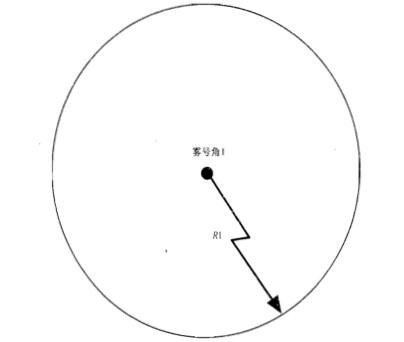
\includegraphics[width=.5\textwidth]{pic/signal_distance.jpg}
            \caption{信号接收点位置分布}
            \label{fig:sig_distance}
        \end{figure}
    \end{itemize}
\end{frame}

\begin{frame}{位置确定}
    \begin{itemize}
        \item \textcolor{red}{三个}信号发射点的位置
        \item 信号接收点与信号发射点的距离
        \item[]
        \begin{figure}
            \centering
            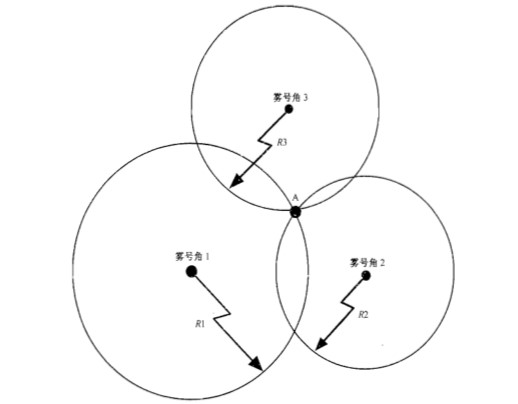
\includegraphics[width=.5\textwidth]{pic/signal_distance_3.jpg}
            \caption{信号接收点位置确定}
            \label{fig:sig_distance_3}
        \end{figure}
    \end{itemize}
\end{frame}

\subsection{坐标系}
\begin{frame}{常用坐标系}
    %\begin{itemize}[<+-| alert@+>]
    \begin{itemize}
        \item 地心地固直角坐标系$\left( \mathrm{ECEF} \right)$
        \begin{itemize}
            \item[] 地心为坐标原点, $OZ$指向北极, $OX$指向参考子午面与地球赤道的交点
        \end{itemize}
        \item 经纬高坐标系$\left( \mathrm{ LLA } \right)$
        \begin{itemize}
            \item[] 地心为坐标原点, 大地高度$h$是过该点到基准椭球面的法线距离
        \end{itemize}
        \item 站心坐标系$\left( \mathrm{ ENU } \right)$
        \begin{itemize}
            \item[] 观测点为坐标原点, 三坐标轴分别指向东, 北, 天方向
        \end{itemize}
    \end{itemize}
\end{frame}

\begin{frame}{坐标变换}
    \begin{itemize}
        \item $\mathrm{LLA} \rightarrow \mathrm{ECEF}$
        \begin{align*}
            x &= \left( N + h \right) \cos \varphi \cos \lambda \\
            y &= \left( N + h \right) \cos \varphi \sin \lambda \\
            z &= \left[ N \left( 1 - \mathrm e ^ 2 \right) + h \right] \sin \varphi
        \end{align*}
        其中,
        \begin{align*}
            \mathrm e &= \sqrt{ 1 - \frac{ b ^ 2 }{ a ^ 2 } } \\
            N &= \frac{ a }{ \sqrt{ 1 - \mathrm e ^ 2 \sin ^ 2 \varphi } }
        \end{align*}
    \end{itemize}
\end{frame}

\begin{frame}{坐标变换}
    \begin{itemize}
        \item $\mathrm{ECEF} \rightarrow \mathrm{LLA}$
        \begin{align*}
            \lambda &= \arctan \frac{ y }{ x } \\
            h &= \frac{ \sqrt{ x ^ 2 + y ^ 2 } }{ \cos \varphi } - N \\
            \varphi &= \arctan \left[ \frac{ z }{ \sqrt{ x ^ 2 + y ^ 2 } }
            \left( 1 - \mathrm e ^ 2 \frac{ N }{ N + h } \right) ^ { -1 }\right]
        \end{align*}
        其中, $h$与$\varphi$组成耦合非线性方程组, 采用迭代方法求解.
    \end{itemize}
\end{frame}

\subsection{卫星星历}
\begin{frame}{星历文件主要参数}
\begin{table}[h!]
    \centering
    \footnotesize
    \caption{星历文件参数}
    \begin{tabular}{ccc}
        \hline
        $t _ { 0e }$ && 星历参考时刻 \\
        $\sqrt{ a }$ && 轨道半长轴的平方根 \\
        $e$ && 轨道离心率 \\
        $i _ 0$ && $t _ { 0e }$时刻轨道倾角 \\
        $\Omega _ 0$ && 升交点经度 \\
        $\omega$ && $t _ { 0e }$时刻近地点幅角 \\
        $M _ 0$ && $t _ { 0e }$时刻平近点角 \\
        $\mathrm d i / \mathrm d t$ && 倾角变化率 \\
        $\mathrm d \Omega / \mathrm d t$ && 升交点经度变化率 \\
        $\Delta n$ && 平均角速度的校正值 \\
        $C _ { uc }$ && 维度幅角余弦修正值 \\
        $C _ { us }$ && 维度幅角正弦修正值 \\
        $C _ { rc }$ && 轨道半径余弦修正值 \\
        $C _ { rs }$ && 轨道半径正弦修正值 \\
        $C _ { ic }$ && 倾角余弦修正值 \\
        $C _ { is }$ && 倾角正弦修正值 \\
        \hline
    \end{tabular}
    \label{tab:ephemeris_para}
\end{table}
\end{frame}

\begin{frame}{计算卫星位置}
    \begin{figure}
        \centering
        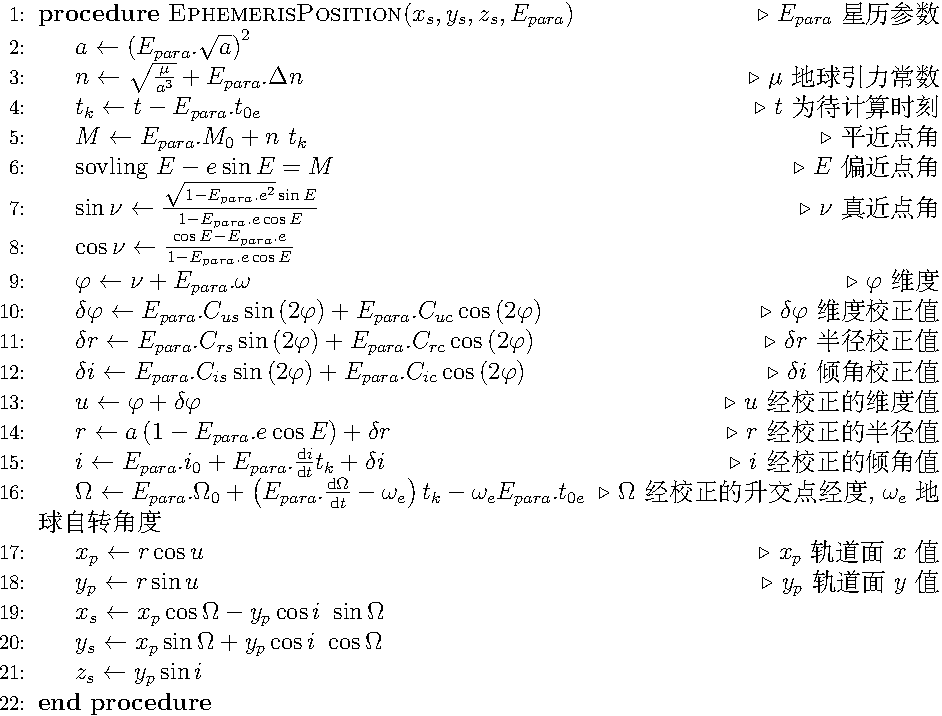
\includegraphics[width = .7\textwidth]{pic/algo_ephemeris.pdf}
        \label{fig:alg_ephemeris}
    \end{figure}
\end{frame}

\subsection{星地距离}
\begin{frame}{记号说明}
    \begin{align*}
        \text{卫星坐标} &: S _ i \left( x ^ { S _ i }, y ^ { S _ i }, z ^ { S _ i } \right), \ i = 1, \ldots, n _ s \\
        \text{接收机坐标} &: R \left( x ^ R, y ^ R, z ^ R \right) \\
        \text{信号离开卫星时刻} &: t _ { S _ i }, \ i = 1, \ldots, n _ s \\
        \text{接收机接收信号时刻} &: t _ R \\
        \text{卫星钟差} &: \delta t _ S \\
        \text{接收机钟差} &: \delta t _ R \\
        \text{接收机载波相位观测值} &: \tilde \varphi _ R ^ { S _ i }, \ i = 1, \ldots, n _ s \\
        \text{光速} &: c
    \end{align*}
\end{frame}

\begin{frame}{测距码}
    \begin{itemize}
        \item R与$S _ i$几何距离$\textcolor{red}{\rho _ R ^ { S _ i }}$
        \begin{align*}
            \textcolor{red}{\rho _ R ^ { S _ i }} &= \sqrt{ \left( x ^ R - x ^ { S _ i } \right) ^ 2
            + \left( y ^ R - y ^ { S _ i } \right) ^ 2
            + \left( z ^ R - z ^ { S _ i } \right) ^ 2 }
        \end{align*}
        \item 信号离开真实时刻$\tau _ { S _ i }$, 接收机接收信号真实时刻$\tau _ R$
        \begin{align*}
            \tau _ { S _ i } &= t _ { S _ i } + \delta t _ S,\
            \tau _ R = t _ R + \delta t _ R
        \end{align*}
        \item 电离层修正值$V _ { \mathrm{ iono, S _ i } } ^ R$, 对流层修正值$V _ { \mathrm{ trop }, S _ i } ^ R$
        \begin{align*}
            \textcolor{red}{\rho _ R ^ { S _ i }} &= c \left( \tau _ R - \tau _ { S _ i } \right)
            + V _ { \mathrm{ iono, S _ i } } ^ R + V _ { \mathrm{ trop }, S _ i } ^ R
        \end{align*}
        \item 伪距${\color{red} \tilde \rho _ R ^ { S _ i } } = c \left( t _ R - t _ { S _ i } \right)$
        \begin{align*}
            {\color{red} \tilde \rho _ R ^ { S _ i } } &= \textcolor{red}{ \rho _ R ^ { S _ i } } - 
            c \textcolor{red}{ \delta t _ R } + c \delta t _ { S _ i }
            - V _ { \mathrm{ iono, S _ i } } ^ R - V _ { \mathrm{ trop }, S _ i } ^ R
        \end{align*}
    \end{itemize}
\end{frame}

\begin{frame}{载波相位}
    \begin{itemize}
        \item 卫星信号载波波长
        \begin{align*}
            \lambda _ 1 &= 19.0 \ \mathrm{ cm },\
            \lambda _ 2 = 24.4 \ \mathrm{ cm }, \
            \lambda _ 3 = 25.5 \ \mathrm{ cm }
        \end{align*}
        \item 接收机收到的载波整周数$\textcolor{red}{N _ R ^ { S _ i }}$
        \begin{align*}
            \textcolor{red}{\tilde \rho _ R ^ { S _ i }} &=
            \lambda \left( \tilde \varphi _ R ^ { S _ i } +
            \textcolor{red}{N _ R ^ { S _ i }} \right) \notag \\
            &= \textcolor{red}{ \rho _ R ^ { S _ i } } - 
            c \textcolor{red}{ \delta t _ R } + c \delta t _ { S _ i }
            - V _ { \mathrm{ iono, S _ i } } ^ R - V _ { \mathrm{ trop }, S _ i } ^ R
        \end{align*}
    \end{itemize}
\end{frame}

% research
\section{研究内容}

\subsection{美化主题}

\begin{frame}{这一份主题与原始的THU Beamer Theme区别在于}
    \begin{itemize}
        \item 顶栏的小点变成一行而不是多行
        \item 中文采用楷书
        \item 剩下我改了啥我也忘了……我16年魔改的,都四年过去了(x
        \item 更多该模板的功能可以参考 \url{https://www.latexstudio.net/archives/4051.html}
        \item 下面列举出了一些Beamer的用法,部分节选自 \url{https://tuna.moe/event/2018/latex/}
    \end{itemize}
\end{frame}

\subsection{如何更好地做Beamer}

\begin{frame}{Why Beamer}
    \begin{itemize}
        \item \LaTeX 广泛用于学术界,期刊会议论文模板
    \end{itemize}
    \begin{table}[h]
        \centering
        \begin{tabular}{c|c}
            Microsoft\textsuperscript{\textregistered}  Word & \LaTeX \\
            \hline
            文字处理工具 & 专业排版软件 \\
            容易上手,简单直观 & 容易上手 \\
            所见即所得 & 所见即所想,所想即所得 \\
            高级功能不易掌握 & 进阶难,但一般用不到 \\
            处理长文档需要丰富经验 & 和短文档处理基本无异 \\
            花费大量时间调格式 & 无需担心格式,专心作者内容 \\
            公式排版差强人意 & 尤其擅长公式排版 \\
            二进制格式,兼容性差 & 文本文件,易读、稳定 \\
            付费商业许可 & 自由免费使用 \\
        \end{tabular}
    \end{table}
\end{frame}

\begin{frame}{排版举例}
    \begin{exampleblock}{无编号公式} % 加 * 
        \begin{equation*}
            J(\theta) = \mathbb{E}_{\pi_\theta}[G_t] = \sum_{s\in\mathcal{S}} d^\pi (s)V^\pi(s)=\sum_{s\in\mathcal{S}} d^\pi(s)\sum_{a\in\mathcal{A}}\pi_\theta(a|s)Q^\pi(s,a)
        \end{equation*}
    \end{exampleblock}
    \begin{exampleblock}{多行多列公式\footnote{如果公式中有文字出现,请用 $\backslash$mathrm\{\} 或者 $\backslash$text\{\} 包含,不然就会变成 $clip$,在公式里看起来比 $\mathrm{clip}$ 丑非常多。}}
        % 使用 & 分隔
        \begin{align}
            Q_\mathrm{target}&=r+\gamma Q^\pi(s^\prime, \pi_\theta(s^\prime)+\epsilon)\\
            \epsilon&\sim\mathrm{clip}(\mathcal{N}(0, \sigma), -c, c)\nonumber
        \end{align}
    \end{exampleblock}
\end{frame}

\begin{frame}
    \begin{exampleblock}{编号多行公式}
        % Taken from Mathmode.tex
        \begin{multline}
            A=\lim_{n\rightarrow\infty}\Delta x\left(a^{2}+\left(a^{2}+2a\Delta x+\left(\Delta x\right)^{2}\right)\right.\label{eq:reset}\\
            +\left(a^{2}+2\cdot2a\Delta x+2^{2}\left(\Delta x\right)^{2}\right)\\
            +\left(a^{2}+2\cdot3a\Delta x+3^{2}\left(\Delta x\right)^{2}\right)\\
            +\ldots\\
            \left.+\left(a^{2}+2\cdot(n-1)a\Delta x+(n-1)^{2}\left(\Delta x\right)^{2}\right)\right)\\
            =\frac{1}{3}\left(b^{3}-a^{3}\right)
        \end{multline}
    \end{exampleblock}
\end{frame}

\begin{frame}{图形与分栏}
    % From thuthesis user guide.
    \begin{minipage}[c]{0.3\linewidth}
        \psset{unit=0.8cm}
        \begin{pspicture}(-1.75,-3)(3.25,4)
            \psline[linewidth=0.25pt](0,0)(0,4)
            \rput[tl]{0}(0.2,2){$\vec e_z$}
            \rput[tr]{0}(-0.9,1.4){$\vec e$}
            \rput[tl]{0}(2.8,-1.1){$\vec C_{ptm{ext}}$}
            \rput[br]{0}(-0.3,2.1){$\theta$}
            \rput{25}(0,0){%
            \psframe[fillstyle=solid,fillcolor=lightgray,linewidth=.8pt](-0.1,-3.2)(0.1,0)}
            \rput{25}(0,0){%
            \psellipse[fillstyle=solid,fillcolor=yellow,linewidth=3pt](0,0)(1.5,0.5)}
            \rput{25}(0,0){%
            \psframe[fillstyle=solid,fillcolor=lightgray,linewidth=.8pt](-0.1,0)(0.1,3.2)}
            \rput{25}(0,0){\psline[linecolor=red,linewidth=1.5pt]{->}(0,0)(0.,2)}
%           \psRotation{0}(0,3.5){$\dot\phi$}
%           \psRotation{25}(-1.2,2.6){$\dot\psi$}
            \psline[linecolor=red,linewidth=1.25pt]{->}(0,0)(0,2)
            \psline[linecolor=red,linewidth=1.25pt]{->}(0,0)(3,-1)
            \psline[linecolor=red,linewidth=1.25pt]{->}(0,0)(2.85,-0.95)
            \psarc{->}{2.1}{90}{112.5}
            \rput[bl](.1,.01){C}
        \end{pspicture}
    \end{minipage}\hspace{1cm}
    \begin{minipage}{0.5\linewidth}
        \medskip
        %\hspace{2cm}
        \begin{figure}[h]
            \centering
            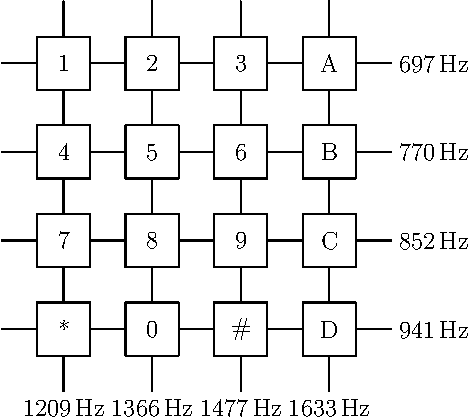
\includegraphics[height=.4\textheight]{pic/dtmf.pdf}
        \end{figure}
    \end{minipage}
\end{frame}

\begin{frame}[fragile]{\LaTeX{} 常用命令}
    \begin{exampleblock}{命令}
        \centering
        \footnotesize
        \begin{tabular}{llll}
            \cmd{chapter} & \cmd{section} & \cmd{subsection} & \cmd{paragraph} \\
            章 & 节 & 小节 & 带题头段落 \\\hline
            \cmd{centering} & \cmd{emph} & \cmd{verb} & \cmd{url} \\
            居中对齐 & 强调 & 原样输出 & 超链接 \\\hline
            \cmd{footnote} & \cmd{item} & \cmd{caption} & \cmd{includegraphics} \\
            脚注 & 列表条目 & 标题 & 插入图片 \\\hline
            \cmd{label} & \cmd{cite} & \cmd{ref} \\
            标号 & 引用参考文献 & 引用图表公式等\\\hline
        \end{tabular}
    \end{exampleblock}
    \begin{exampleblock}{环境}
        \centering
        \footnotesize
        \begin{tabular}{lll}
            \env{table} & \env{figure} & \env{equation}\\
            表格 & 图片 & 公式 \\\hline
            \env{itemize} & \env{enumerate} & \env{description}\\
            无编号列表 & 编号列表 & 描述 \\\hline
        \end{tabular}
    \end{exampleblock}
\end{frame}

\begin{frame}[fragile]{\LaTeX{} 环境命令举例}
    \begin{minipage}{0.5\linewidth}
\begin{lstlisting}[language=TeX]
\begin{itemize}
  \item A \item B
  \item C
  \begin{itemize}
    \item C-1
  \end{itemize}
\end{itemize}
\end{lstlisting}
    \end{minipage}\hspace{1cm}
    \begin{minipage}{0.3\linewidth}
        \begin{itemize}
            \item A
            \item B
            \item C
            \begin{itemize}
                \item C-1
            \end{itemize}
        \end{itemize}
    \end{minipage}
    \medskip
    \pause
    \begin{minipage}{0.5\linewidth}
\begin{lstlisting}[language=TeX]
\begin{enumerate}
  \item 巨佬 \item 大佬
  \item 萌新
  \begin{itemize}
    \item[n+e] 瑟瑟发抖
  \end{itemize}
\end{enumerate}
\end{lstlisting}
    \end{minipage}\hspace{1cm}
    \begin{minipage}{0.3\linewidth}
        \begin{enumerate}
            \item 巨佬
            \item 大佬
            \item 萌新
            \begin{itemize}
                \item[n+e] 瑟瑟发抖
            \end{itemize}
        \end{enumerate}
    \end{minipage}
\end{frame}

\begin{frame}[fragile]{\LaTeX{} 数学公式}
    \begin{columns}
        \begin{column}{.55\textwidth}
\begin{lstlisting}[language=TeX]
$V = \frac{4}{3}\pi r^3$

\[
  V = \frac{4}{3}\pi r^3
\]

\begin{equation}
  \label{eq:vsphere}
  V = \frac{4}{3}\pi r^3
\end{equation}
\end{lstlisting}
        \end{column}
        \begin{column}{.4\textwidth}
            $V = \frac{4}{3}\pi r^3$
            \[
                V = \frac{4}{3}\pi r^3
            \]
            \begin{equation}
                \label{eq:vsphere}
                V = \frac{4}{3}\pi r^3
            \end{equation}
        \end{column}
    \end{columns}
    \begin{itemize}
        \item 更多内容请看 \href{https://zh.wikipedia.org/wiki/Help:数学公式}{\color{purple}{这里}}
    \end{itemize}
\end{frame}

\begin{frame}[fragile]
    \begin{columns}
        \column{.6\textwidth}
\begin{lstlisting}[language=TeX]
    \begin{table}[htbp]
      \caption{编号与含义}
      \label{tab:number}
      \centering
      \begin{tabular}{cl}
        \toprule
        编号 & 含义 \\
        \midrule
        1 & 4.0 \\
        2 & 3.7 \\
        \bottomrule
      \end{tabular}
    \end{table}
    公式~(\ref{eq:vsphere}) 的
    编号与含义请参见
    表~\ref{tab:number}。
\end{lstlisting}
        \column{.4\textwidth}
        \begin{table}[htpb]
            \centering
            \caption{编号与含义}
            \label{tab:number}
            \begin{tabular}{cl}\toprule
                编号 & 含义 \\\midrule
                1 & 4.0\\
                2 & 3.7\\\bottomrule
            \end{tabular}
        \end{table}
        \normalsize 公式~(\ref{eq:vsphere})的编号与含义请参见表~\ref{tab:number}。
    \end{columns}
\end{frame}

\begin{frame}{作图}
    \begin{itemize}
        \item 矢量图 eps, ps, pdf
        \begin{itemize}
            \item METAPOST, pstricks, pgf $\ldots$
            \item Xfig, Dia, Visio, Inkscape $\ldots$
            \item Matlab / Excel 等保存为 pdf
        \end{itemize}
        \item 标量图 png, jpg, tiff $\ldots$
        \begin{itemize}
            \item 提高清晰度,避免发虚
            \item 应尽量避免使用
        \end{itemize}
    \end{itemize}
    \begin{figure}[htpb]
        \centering
        
\includegraphics[width=0.2\linewidth]{pic/Tsinghua_University_Logo.eps}
        \caption{这个校徽就是矢量图}
    \end{figure}
\end{frame}

% schedule
% RTKLIB source file
\section{RTKLIB源程序}
\begin{frame}{单点定位RTCM}
    \begin{itemize}
        \item RTCM file
        \begin{figure}
            \centering
            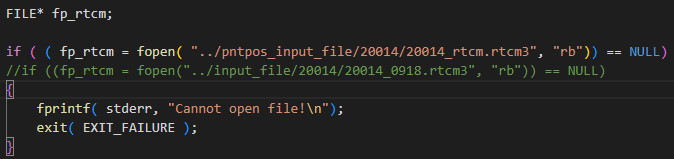
\includegraphics[width=.5\textwidth]{pic/rtcm_file.png}
            \caption{RTCM文件}
            \label{fig:rtcm_file}
        \end{figure}
        \item 单点定位配置
        \begin{figure}
            \centering
            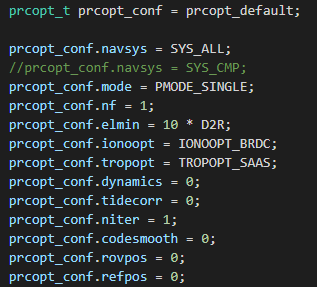
\includegraphics[width=.3\textwidth]{pic/prcopt_config.png}
            \caption{单点定位配置}
            \label{fig:pnt_config}
        \end{figure}
    \end{itemize}
\end{frame}

\begin{frame}{nav数据结构初始化声明}
    \begin{figure}
        \centering
        
\includegraphics[width=.5\textwidth]{pic/nav_data_memset.png}
        \caption{nav数据}
        \label{fig:nav_data}
    \end{figure}
\end{frame}

\begin{frame}{求解流程}
    \begin{figure}
        \centering
        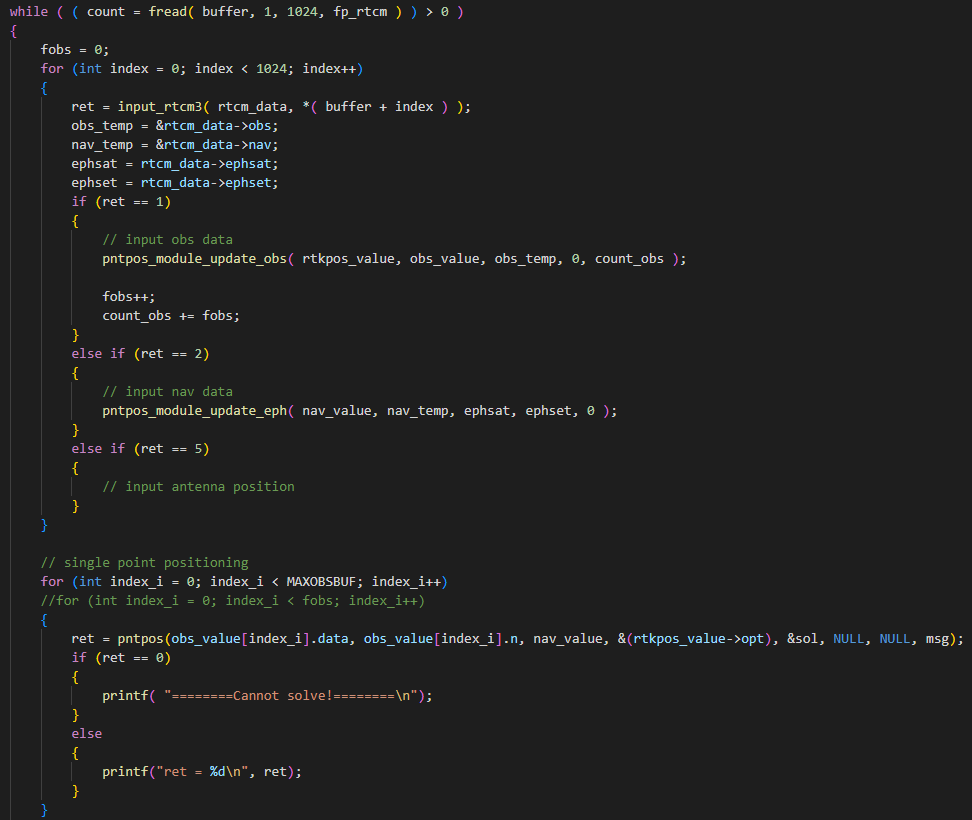
\includegraphics[width=.5\textwidth]{pic/pntpos_process.png}
        \caption{逻辑流程}
        \label{fig:pntpos_process}
    \end{figure}
\end{frame}

\section{Future work}
\begin{frame}{Future}
    \begin{itemize}
        \item LAMBDA算法文献调研
        \item 离散型优化算法
        \item 网平差算法
        \item 国产化平台JAVA调用C程序.so文件打包
    \end{itemize}
\end{frame}

\section{参考文献}

\begin{frame}[allowframebreaks]
    \nocite{*}
    \bibliography{ref}
    \bibliographystyle{plain}
    % 如果参考文献太多的话,可以像下面这样调整字体:
    % \tiny\bibliographystyle{alpha}
\end{frame}

% end page
{
\setbeamertemplate{background} 
{
    
\includegraphics[width=\paperwidth,height=\paperheight]{pic/front_page.jpg}
}
\begin{frame}
    \begin{center}
        {\Huge\calligra Thanks for your attention!}
    \end{center}
\end{frame}
}

\end{document}